\documentclass{article}

\usepackage{graphicx} % for images
\usepackage{amsmath} % for math
\usepackage{amssymb} % for \mathbb
\usepackage{siunitx} % for \SI, \num
\usepackage{hyperref} % for \url{}

% This stuff is for figures
\usepackage{float}
\DeclareGraphicsExtensions{.pdf, .png, .jpg}

% coloring of links for PDF format
\hypersetup{
    colorlinks=true,
    urlcolor=blue,
    linkcolor=black
}

% \c command redefinition (for monospaced font)
\renewcommand{\c}[1]{\texttt{#1}}
% \today command re-definition
%https://tex.stackexchange.com/questions/112932/today-month-as-text
\renewcommand{\today}{\ifnum\number\day<10 0\fi \number\day \space%
\ifcase \month \or January\or February\or March\or April\or May%
\or June\or July\or August\or September\or October\or November\or December\fi\space%
\number \year} 

\begin{document}

\noindent
Rodrigo Becerril Ferreyra\\
E E 381 Section 12\\
Lab 5\\
\today

\addcontentsline{toc}{section}{Introduction}
\section*{Introduction} The purpose of this lab is to
experience random sampling from a population, and using
a sample to estimate properties about the entire population.
Specifically, we were tasked with creating samples \(\bar{X}\)
of various sizes, finding their mean \(\mu_{\bar{X}}\), and
comparing their values to the population mean \(\mu\) (known
beforehand).

The probability that
the population mean \(\mu\) is in between two values
satisfies the following equation:
\begin{equation}
    P\left( \bar{X} - z \frac{\hat{S}}{\sqrt{n}} \le \mu \le \bar{X} + z \frac{\hat{S}}{\sqrt{n}} \right) = F(z),
\end{equation} where \(\bar{X} \pm z \frac{\hat{S}}{\sqrt{n}}\)
are the upper and lower bounds of \(\mu\) and \(F(z)\)
represents the cumulative distribution function (CDF) of
the distribution in question. \(F(z)\) represents
the probability that \(\mu\) lies between the two bounds.
Common choices for \(F(z)\) are \num{0.95} and \num{0.99};
the values of \(z\) can be found using common tables,
and are listed below for convenience.
\begin{table}[H]
    \centering
    \begin{tabular}{|c|c|c|}
        \hline
        \( F(z) \) & \begin{tabular}[c]{@{}c@{}}Standard Normal Distribution\\ \( \mu = 0, \sigma = 1 \)\end{tabular} & \begin{tabular}[c]{@{}c@{}}Student's t-Distribution\\ \( \nu = 4 \)\end{tabular} \\ \hline
        0.95 & \( z = 1.96 \) & \( z = 2.78 \) \\ \hline
        0.99 & \( z = 2.58 \) & \( z = 4.60 \) \\ \hline
    \end{tabular}
    \caption{Table of common values for \(F(z)\).}
    \label{table:CDF}
\end{table}

The population for this lab was generated using a normal
distribution with a mean of \(\mu = \SI{55}{\gram}\) and a
standard deviation of \(\sigma = \SI{5}{\gram}\). The population
size is \num{1500000}.

\section{Problem 1}
\subsection{Question} In this problem, the task is to take
200 samples, with each sample's size increasing each time
(for example, the first sample has a size of 1, the second
sample has a size of 2, etc.). The mean of each sample was taken,
and plotted against its sample size. It is worth noting that
the sampling was done with replacement; ergo, it is possible
that a certain value was selected more than once.

\subsection{Results} The graphs of the sample means vs sample
sizes compared with the theoretical upper and lower bounds
given by \(g_{99}(\text{size}) = \mu \pm \frac{2.58\sigma}{\sqrt{\text{size}}} \)
and \(g_{95}(\text{size}) = \mu \pm \frac{1.96\sigma}{\sqrt{\text{size}}} \)
are listed below\footnote{The values 2.58 and 1.96 were
selected from Table \ref{table:CDF}.}. Note that the
data (points on the plot) are the same; the only difference
between the two plots are the upper and lower bounds of the mean.
For the first plot, it can be assumed that 99\% of the points
are within the boundaries; for the second plot, 95\% of the
points are within the boundaries.

\begin{figure}[H]
    \centering
    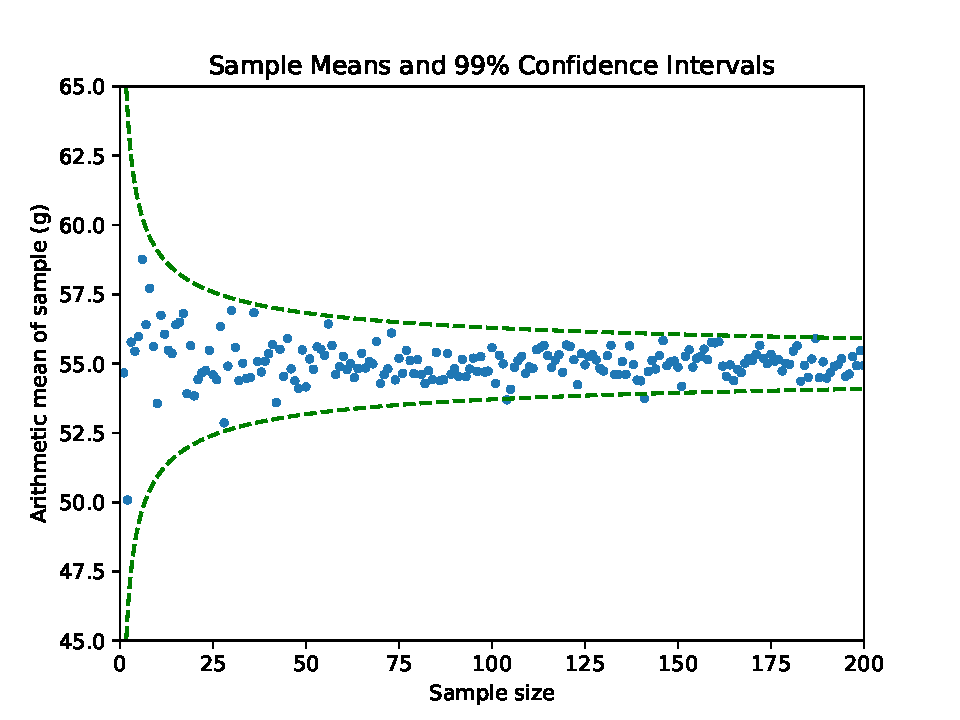
\includegraphics[height=125pt]{Images/Figure2} 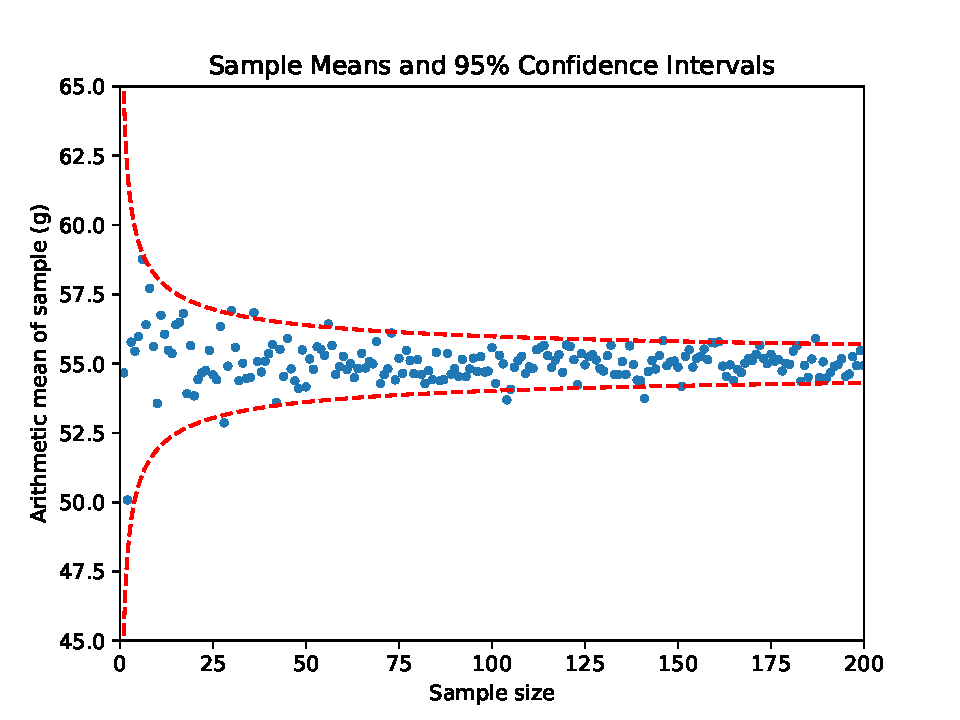
\includegraphics[height=125pt]{Images/Figure1}
    \caption{Scatter plots of sample mean vs. sample size.}
    \label{Prob1:plots}
\end{figure}

Note that as the sample size approaches infinity, the sample mean
approaches \(\mu\). This problem took about \SI{0.168}{s}
to complete.

\section{Problem 2}
\subsection{Question} In this problem, the task is to compare
the use of \(z\)-values (see Table \ref{table:CDF}) in order
to estimate the upper and lower limits of the population mean.
This was done for various sample sizes, using
both normal and Student's t-distributions.

In this lab, a large sample size is defined as having greater
than or equal to 30 elements, while a small sample size is
defined as having less than 30 elements. For small sample
sizes, the t-distribution is a better estimator of the
population mean, while the normal distribution is a better
estimator for large samples. This can be seen in
Table \ref{table:prob2}.

The process to obtain the values in Table \ref{table:prob2}
is as follows: first, the mean and sample standard
deviation of the sample were obtained using the following
equations:
\begin{gather}
    \bar{X} = \frac1{\text{size}} \sum X \label{mean}\\
    \hat{S} = \sqrt{\frac1{\text{size} - 1} \sum (X - \bar{X})^2}
    \label{std}
\end{gather} Using the mean calculated in \eqref{mean} and the
sample standard deviation calculated in \eqref{std}, we can
calculate the upper and lower bounds as follows:
\begin{gather}
    \mu_\text{lower} = \bar{X} - z\frac{\hat{S}}{\sqrt{n}}
    \label{mu lower}\\
    \mu_\text{upper} = \bar{X} + z\frac{\hat{S}}{\sqrt{n}}
    \label{mu upper}
\end{gather} where \(z\) is taken appropriately from
Table \ref{table:CDF}.

In Problem 2, \num{10000} tests were conducted for each sample
size. If the expression
\(\mu \in [\mu_\text{lower}, \mu_\text{upper}]\)
holds true, then that test is considered a success; if not,
then the test is a failure. The ratio of the number of
successes to the total number of tests is shown in Table 
\ref{table:prob2}.

\subsection{Results}
\begin{table}[H]
    \centering
    \begin{tabular}{|c|c|c|c|c|}
        \hline
        \begin{tabular}[c]{@{}c@{}}Sample size\\ \( (n) \)\end{tabular} & \begin{tabular}[c]{@{}c@{}}\( F(z) = 0.95 \)\\ Normal\end{tabular} & \begin{tabular}[c]{@{}c@{}}\( F(z) = 0.99 \) \\ Normal\end{tabular} & \begin{tabular}[c]{@{}c@{}}\( F(z) = 0.95 \)\\ Student's t\end{tabular} & \begin{tabular}[c]{@{}c@{}}\( F(z) = 0.99 \)\\ Student's t\end{tabular} \\ \hline
        5 & 87.35\% & 93.48\% & 94.79\% & 98.94\% \\ \hline
        40 & 94.18\% & 98.59\% & 99.10\% & 100.0\% \\ \hline
        120 & 94.65\% & 98.91\% & 99.27\% & 100.0\% \\ \hline
    \end{tabular}
    \caption{Success rate for different sample sizes.}
    \label{table:prob2}
\end{table}

According to the definition of small and large sample sizes
for this lab, it is inappropriate to use a value of \(z\)
associated with the normal CDF for \(\text{size}=5\);
this can be seen clearly, as \num{0.8735} is not close
to \num{0.95}, and \num{0.9348} is not close to \num{0.99}.
The values for the Student's t-distribution are much closer
(\num{0.9479} is close to \num{0.95} and \num{0.9894} is close
to \num{0.99}), which makes it the superior choice for small
sample sizes. This fact is reversed, however, when
\(\text{size} = 40\) and \(\text{size} = 120\). In these cases,
the normal distribution values are much closer to their expected
values, but the t-distribution values are much higher,
and sometimes these values are 1, meaning that, in these cases,
\(\mu_\text{lower}\) was very small and \(\mu_\text{upper}\) was
very big such that they tell no information on
the location of the population mean;
in other words,
the range of
\([\mu_\text{lower}, \mu_\text{upper}]\) is too broad.
Therefore, it is best to use a normal distribution CDF value
for large sample sizes.

This problem took about \SI{6.95}{s} to compute.

\section{Media} The following is an image displaying
the output of the \c{main.py} file.

\begin{figure}[H]
    \centering
    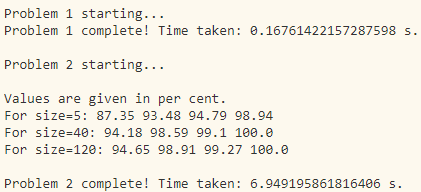
\includegraphics[width=\textwidth]{Images/output}
    \caption{Output from source file.}
    \label{figure:output}
\end{figure}

\end{document}
\footnote{This
function is given by \(F(z) = \frac12 \left[1 + \operatorname{erf}\left( \frac{z}{\sqrt{2}} \right)\right]\),
where \(\operatorname{erf}\) is the error function.}
